\documentclass{beamer}
\usepackage{graphicx}

\mode<presentation>{\usetheme{Warsaw}}
\title{Moogle!}
\author{Amalia Beatriz Valiente Hinojosa\\C-112}
\institute{ Facultad de Matem\'atica y Computaci\'on, Universidad de La Habana}
\date{}

\begin{document}
\begin{frame}
{\titlepage}
\end{frame}

\begin{frame}
    \frametitle{\'Indice}
    \begin{itemize}
        \item ¿Qu\'e es Moogle!?
        \item Estructura de Moogle!
        \item Manual de b\'usqueda.
    \end{itemize}

\end{frame}

\begin{frame}
    \frametitle{¿Qu\'e es Moogle!?}
    \Large Moogle! es una aplicaci\'on cuyo prop\'osito es buscar inteligentemente y de forma eficiente un texto en un conjunto de documentos.\\ Para su funcionamiento fue emplado el modelo de espacio vectorial, un modelo algebr\'aico utilizado, entre otras cosas, para el c\'alculo de relevancia de informaci\'on otorgando cierto valor de similitud entre los documentos y la consulta.
\end{frame}

\begin{frame}
    \frametitle{Estructura de Moogle!}
    \Large Para la construcci\'on del buscador se elaboraron cuatro clases:
    \begin{itemize}
        \item Moogle.
        \item Processor.
        \item TF-IDF
        \item Query.
    \end{itemize}
    
\end{frame}

\begin{frame}
\frametitle{Estrutura de Moogle!}
  \textbf{\Large Moogle:}\\
  \Large En esta clase se encuentra el m\'etodo principal, \underline{Query}, este m\'etodo devuelve los documentos resultantes de la b\'usqueda.\\
  \textbf{\Large Processor:}\\
  \Large Esta clase contiene m\'etodos encargados de:
  \begin{itemize}
    \item Normalizar los documentos.
    \item Separar y almacenar los documentos en diccionarios.
  \end{itemize}
\end{frame}

\begin{frame}
    \frametitle{Estructura de Moogle!}
\textbf{\Large Query:}\\
 \Large En esta clase se encuentran los m\'etodos encargados de:\\
 \begin{itemize}
    \item Normalizar el contenido de la query eliminando caracteres especiales como tildes, etc.
    \item Calcular el peso de las palabras de la query mediante la f\'ormula:\\
    \begin{equation}
        QW_i = ( b +(1-b)\cdot \frac{freq_i}{maxfreq})\times idf_i
    \end{equation}
    
 \end{itemize}
\end{frame}

\begin{frame}
    \frametitle{Estructura de Moogle!}
   \Large Donde:\\ \textbf{QW} (i) = peso de la palabra (i) de la query.\\
   \textbf{b} = t\'ermino de suavizado, cuyo valor es 0.5.\\ \textbf{freq} (i) = cantidad de veces que se repite el t\'ermino (i).\\ \textbf{maxfreq} = el valor
   del t\'ermino que m\'as se repite en la query.\\ \textbf{idf} = la frecuencia inversa del t\'ermino (i) de la query.
\end{frame}

\begin{frame}
    \frametitle{Estructura de Moogle!}
    \textbf{\Large TF-IDF:}\\ \Large Esta clase contiene los m\'etodos encargados de:\\
    \begin{itemize}
        \item Calcular el peso de las palabras de los documentos mediante la f\'ormula del tfxidf:\\
         \begin{equation}
            W_{t,d} = tf_{t,d}\times idf_t
         \end{equation}
         \Large Donde:\\
          \begin{itemize}
            \item \textbf{w} (t,d) = peso del t\'ermino t en documento d.
         \end{itemize}
    \end{itemize}
\end{frame}

\begin{frame}
    \frametitle{Estructura de Moogle!}
    \begin{itemize}
        \item Continuando con el peso de las palabras:\\
        \begin{itemize}
            \item \begin{equation}
                tf_{t,d} = \frac{freq_{t,d}}{maxfreq_d}
                \end{equation}
                \Large Donde:\\
                \begin{itemize}
                    \item \textbf{tf} (t,d) = cantidad de veces que se repite el t\'ermino t en el documento d.
                    \item \textbf{maxfreq} (d) = el valor del t\'ermino que m\'as se repite en el documento d.
                \end{itemize}
            \item \begin{equation}
                  idf_t = \log_{10} (\frac {N} {n_t})
            \end{equation}
            \Large Donde:\\ 
            \begin{itemize}
                \item \textbf{idf} (t) = frecuencia inversa del t\'ermino t.
                \item \textbf{N} = cantidad de documentos en la base de datos.
                \item \textbf{n} (t) = cantidad de documentos en los que aparece el t\'ermino t.
            \end{itemize}
         \end{itemize}
    \end{itemize}
\end{frame}

\begin{frame}
    \frametitle{Estructura de Moogle!}
   \begin{itemize}
    \item Hallar el valor de similtud que hay entre los documentos y la query mediante la f\'ormula de similitud de coseno:
     \begin{equation}
      sim_{d,q} = \frac{\vec{d} \cdot \vec{q}}{|\vec{d}|\cdot |\vec{q}|}
     \end{equation}
     \begin{center}
         \tiny El denominador es el resultado de multiplicar la norma de los vectores documento y query.
     \end{center}
      \item Almacenar en un diccionario los documentos ordenados en funci\'on de la similitud. 
      \item Encontrar una porci\'on del texto resultante donde sale al menos una palabra de la query, a esto se le llama Snippet.
   \end{itemize}
\end{frame}

\begin{frame}[fragile]
    \frametitle{Manual de b\'usqueda}
    \begin{figure}
    \Large Para efectuar una consulta en Moogle! basta con escribir fragmentos o el nombre del documento que se quiere encontrar y dar click en el bot\'on azul que se encuentra a la derecha de la barra de consulta.\\
    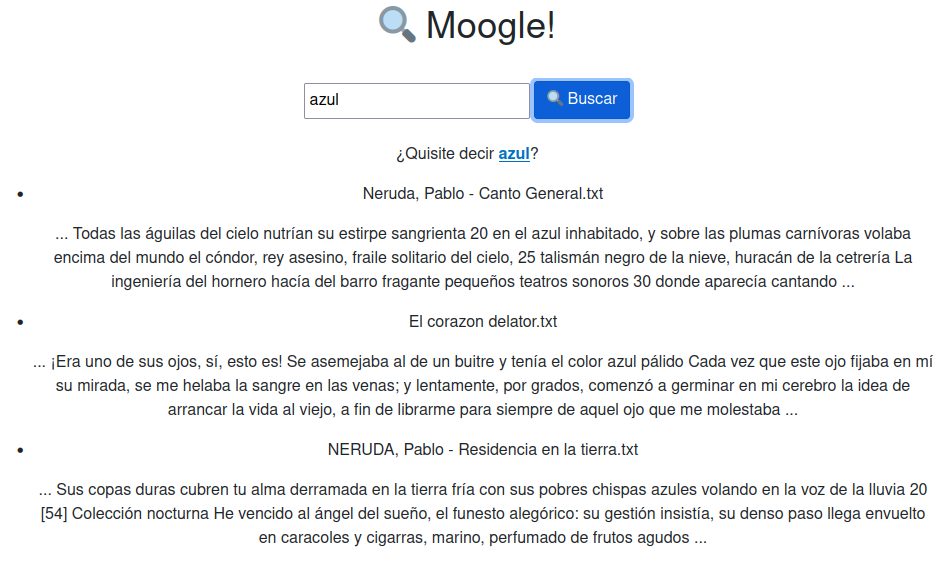
\includegraphics[width=0.7 \linewidth]{ejemplo.png}
    \end{figure}
\end{frame}

\end{document}